\documentclass[twocolumn]{aastex62}
\usepackage[latin1]{inputenc}
\usepackage[english]{babel}
\usepackage{amsmath}
\usepackage{amsfonts}
\usepackage{amssymb}
\usepackage{makeidx}
\usepackage{graphicx}
\usepackage[left=2cm,right=2cm,top=2cm,bottom=2cm]{geometry}

\newcommand{\Ms}{{\rm M}_\odot}
\newcommand{\au}{{\rm AU}}
\newcommand{\gw}{{\rm GW}}
\newcommand{\ibh}{{\rm IMBH}}
\newcommand{\inn}{{\rm in}}
\newcommand{\out}{{\rm out}}
\newcommand{\bh}{{\rm BH}}
\newcommand{\bhu}{{\rm BH1}}
\newcommand{\bhd}{{\rm BH2}}
\newcommand{\ARGdf}{\texttt{ARGdf}}
\newcommand{\ARCHAIN}{\texttt{ARCHAIN}}

\graphicspath{{./}{./}}

\received{}
\revised{revised to \today}
\accepted{}

\submitjournal{ApJ (not yet ..)}

\shorttitle{IMRIs in GCs}
\shortauthors{Arca Sedda, M. and Amaro-Seoane, P.}

\begin{document}

\title{Intermediate mass ratio formation in globular clusters: perspectives for LISA sources formation}

\correspondingauthor{Manuel Arca Sedda}
\email{m.arcasedda@gmail.com}

\author{Manuel Arca Sedda and Pau Amaro-Seoane}
\affil{Zentrum f\"{u}r Astronomie der Universit\"{a}t  Heidelberg\\
Astronomisches Rechen-Institut\\
M\"onchhofstrasse 12-14\\
Heidelberg, D-69120, DE}
\affil{...}

\begin{abstract}
We study the formation and evolution of intermediate mass ratio inspirals (IMRIs) triggered by the interactions between stellar black holes and an intermediate black hole (IMBH) inhabiting. We show the probability for an IMRI to form is an increasing function of the IMBH mass, representing a viable channel for the development of gravitational wave sources that can be possibly observed with the future generation of detectors.
\end{abstract}

\keywords{black holes - supermassive black holes - galactic nuclei - gravitational waves}


\section{Introduction}

Intermediate mass black holes, with masses in the range $10^2-10^5\Ms$, might represent the missing link between stellar and supermassive mass black holes. Dense stellar systems, such as globular clusters (GCs), are thought to be ideal factories for IMBH production via formation and collapse of a very massive stars through stellar collisions \citep{zwart02, giersz15, mapelli16} or via multiple interactions and mergers between stars and stellar-mass BHs \citep{giersz15}. Unfortunately, a striking observational evidence for the presence of IMBHs inhabiting GCs is still missing due to the the little dynamical effects that these objects have on their surroundings. Indeed, models suggest that several processes can mimic an IMBH, like anisotropies in the GC kinematical properties \citep{zocchi}, or the presence of a dense cluster of stellar mass BHs that dominate the inner cluster centre \citep{AAG18a,AAG18b,AS16,vandermarel10}. Nevertheless, a few observational IMBHs candidates have been found for Galactic GCs \citep{noyola10,lu13,lanzoni13,kiziltan17} and their mass and influence radius might be possibly connected with the host cluster observational properties \citep{AAG18a}. Due to this, finding an unique way to unravel the presence of IMBHs in GCs represents one of the most interesting challenges in modern astronomy. Beside this, the presence of an IMBH sitting in the centre of a dense cluster represents a scenario particularly appealing from the perspectives of gravitational waves (GW) astronomy. Indeed, a compact remnants orbiting the IMBH can enter a regime where GWs emission dominates, leading to the formation of an intermediate mass-ratio inspiral \citep[IMRI,][]{konstantinidis13,haster16,leigh14}, a class of sources possible audible with the next generation of GW observatories like LISA \citep{seoane07,amaro12,seoane18}

However, in the highly dense regions that characterize star clusters centres, the formation of IMRIs is not a smooth process. Indeed, due to the continuous interactions with stars, an IMRI ``progenitor'', namely a tight IMBH-BH binary, might be subjected to strong perturbation induced, for instance by a passing-by BH. The three-body interaction involving the IMBH and the two BHs can lead to a variety of end states, including the formation of an IMRI, a stellar BH binary, the ejection of one BH, or even both, or the development of a head-on collision. 

Quantifying the branching ratio for IMRIs formation constitute a fundamental step to assess the probability to observe in the GW domain these sources in the coming future. 

In this paper, we explore the evolution of an IMRI progenitor subjected to the interaction with a perturber making use of three-body simulations that include the host cluster potential and post-Newtonian corrections up to the 2.5 order. We show that the probability for an IMRI to develop is $\sim 15\%$ on average, and its an increasing function of the IMBH mass. 
The maximum probability is achieved for IMBHs with mass $\gtrsim 10^5\%$, for which this quantity rises up to $30\%$.

The paper is organized as follows: in Section \ref{num} we present and summarize the numerical setup used to model the IMBH - BH interaction, in Section \ref{} we discuss the main properties of the simulations outputs, and the implications for GW astronomy, while Section \ref{} is devoted to the results summary and conclusions. 


\section{Initial conditions}
\label{num}

In order to quantify the probability for an IMBH-BH binary to develop and turn into an IMRI via interaction with an external perturber, we perform a series of direct N-body simulations modelling an IMBH-BH-BH triple system placed at the centre of an external gravitational field, which is meant to model the host cluster potential.

The model can be schematized through different parameters that can be gathered in four groups:
\begin{itemize}
\item the IMBH-BH binary depends on the IMBH and BH masses, $M_\ibh$ and $M_\bhu$, the binary semi-major axis $a_\inn$ and its eccentricity $e_\inn$. We refer to this system as the {\it inner binary};
\item the third BH orbiting the inner binary, as well, depends on its mass $M_\bhd$, semi-major axis $a_\out$, eccentricity $e_\out$. We refer to the (IMBH+BH)+BH system as the {\it outer binary}. The inner and outer binaries are characterized by the mutual inclination angle $i$;
\item the host cluster is modelled via Dehnen density profiles, thus being characterized by total mass, $M_c$, scale radius, $r_c$, and the inner slope of the density profile $\gamma$.
\end{itemize}

We develop two simulations series, namely model 1 and model 2, aiming at disentangling the effect of the orbital parameters and the IMBH mass on IMRIs development. The totality of the simulations consists of 929 runs. 

We select four different values for the IMBH mass, ${\rm Log}(M_\ibh/\Ms) = 2,3,4,5$, with the aim to understand how this quantity affects IMRIs formation. In model 1, the IMBH mass is assumed to be one of the four values above, while in model 2 we select the IMBH mass across the $10^2-10^5\Ms$ range, assuming a flat distribution in the logarithm.

The stellar BH masses are selected assuming a power-law mass distribution, $f(M_\bh)\propto M_\bh^{-s}$, with $s = 2.2$, limited between $M_{\rm min} = 10\Ms$ and $M_{\rm max} = 30\Ms$.

The inner binary semi-major axis, $a_\inn$, is drawn accordingly to a distribution flat in the logarithm between $10$ and $315$ AU. For the outer orbit, we selected $a_\out$ in the range $20 - 630$ AU (model 1) and $50 - 1500 $ AU (model 2), assuming a logarithmically flat distribution.
Moreover, we assume a thermal distribution for the eccentricity, $P(e){\rm d}e = 2e{\rm d}e$. The mutual orbital inclination $i$ is selected randomly between $0$ and $\pi$.
The simulations are halted either if one of the two BH merge with the IMBH, if one of the BHs is ejected away of if the simulated time exceeds $t = 5\times 10^5 P_\inn$, where $P_\inn$ represents the initial value of the inner binary orbital period. 
The main properties of our runs are summarized in Table \ref{t1}.

\begin{table*}
\caption{Main properties of our models}
\begin{center}
\begin{tabular}{ccccccccc}
\hline
model   & $f(M_\ibh)$ & $M_\ibh$ & $f(M_\bh)\propto M_\bh^{-s}$ & $M_\bh$ & $a_\inn$ & $e_\inn$ & $a_\out$ & $e_\out$ \\ 
        &             & $\Ms$    &            & $\Ms$   & $\au$    &          & $\au$    &          \\
\hline 
1 & Log, Discrete & $10^2-10^5$ & $s=2.2$ & $10-30$ & $10-315$ & Thermal & $20-630$ & Thermal \\
2 & Log, Continuous & $10^2-10^5$ & $s=2.2$ & $10-30$ & $10-315$ & Thermal & $50-1500$ & Thermal \\
\hline
\end{tabular}
\end{center}
\label{t1}
\end{table*}


The cluster total mass is calculated via the scaling relation \citep{AS16}
\begin{equation}
{\rm Log} M_c = {\rm Log} M_\ibh + 2.23;
\label{mcmibh}
\end{equation}
the cluster length scale $r_c$ is selected randomly between 0.2 and 1.0 pc. We also assume a flat distribution for the cluster density slope, assuming $\gamma \leq 1$.

Given the choices above, the IMBH influence radius can be easily connected with the cluster structural properties, namely
\begin{equation}
R_{\rm inf} = \frac{GM_\ibh}{\sigma} = \frac{M_\ibh}{M_c}R_{\rm hm},
\end{equation}
where we substituted the cluster velocity dispersion $\sigma$ with its value calculated at the cluster half-mass radius $R_{\rm hm}$, which in turn can be expressed in terms of the length scale and slope as
\begin{equation}
R_{\rm hm} = r_c(2^{1/(3-\gamma)}-1)^{-1}.
\end{equation} 
Therefore, the IMBH influence radius in our models is given by 
\begin{equation}
R_{\rm inf} = \mu r_c(2^{1/(3-\gamma)}-1)^{-1},
\end{equation}
where $\mu = M_\ibh/M_c = 0.0058$ via Equation \ref{mcmibh}.

As shown in Figure \ref{corerad}, the limiting values set for the inner and outer binaries are in almost all the cases, below the IMBH influence radius, with a few exceptions. Within this regions, particles are expected to be gravitationally bound to the IMBH, and their orbits are most-likely Keplerian, although on the long-term the self-interaction among all the orbits can drive a reorientation of the angular momenta, a phenomenon known as vector resonant relaxation \cite{}.

\begin{figure}
\centering 
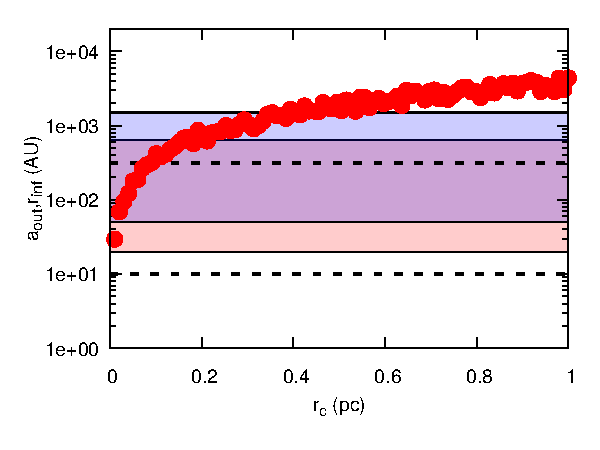
\includegraphics[width=8cm]{core_influ}
\caption{IMBH influence radius (red dots) as a function of the cluster core radius. The red and blue regions encompass the ranges allowed for the outer binary semi-major axis in model 1 and 2, respectively. The two dotted lines enclose the allowed range for the inner binary semi-major axis, instead.}
\label{corerad}
\end{figure}

Our models are a simplified approximation of what occur in the innermost regions of a real star cluster harbouring an IMBH. Indeed, an IMBH is expected to interact continuously with cluster stars, rather than with only a few of them. Assuming a typical IMBH mass of $M_\ibh = 10^3\Ms$ inhabiting a cluster with core radius $r_c = 0.5$ pc and density slope $\gamma \sim 0.2$, it is simple to show that the cluster mass enclosed within the IMBH influence radius is limited to $\simeq 100 \Ms$. Since heavy compact remnants are expected to dominate the stellar population in the deepest cluster region due to mass segregation, we expect that such stellar mass is mostly comprised of a few stellar mass BHs and neutron stars.

%If only two BHs are sufficiently close to interact with the IMBH, as we model in the following, there are several possible outcomes, which are schematized in Figure \ref{sketch}. 
%\begin{figure*}
%\centering
%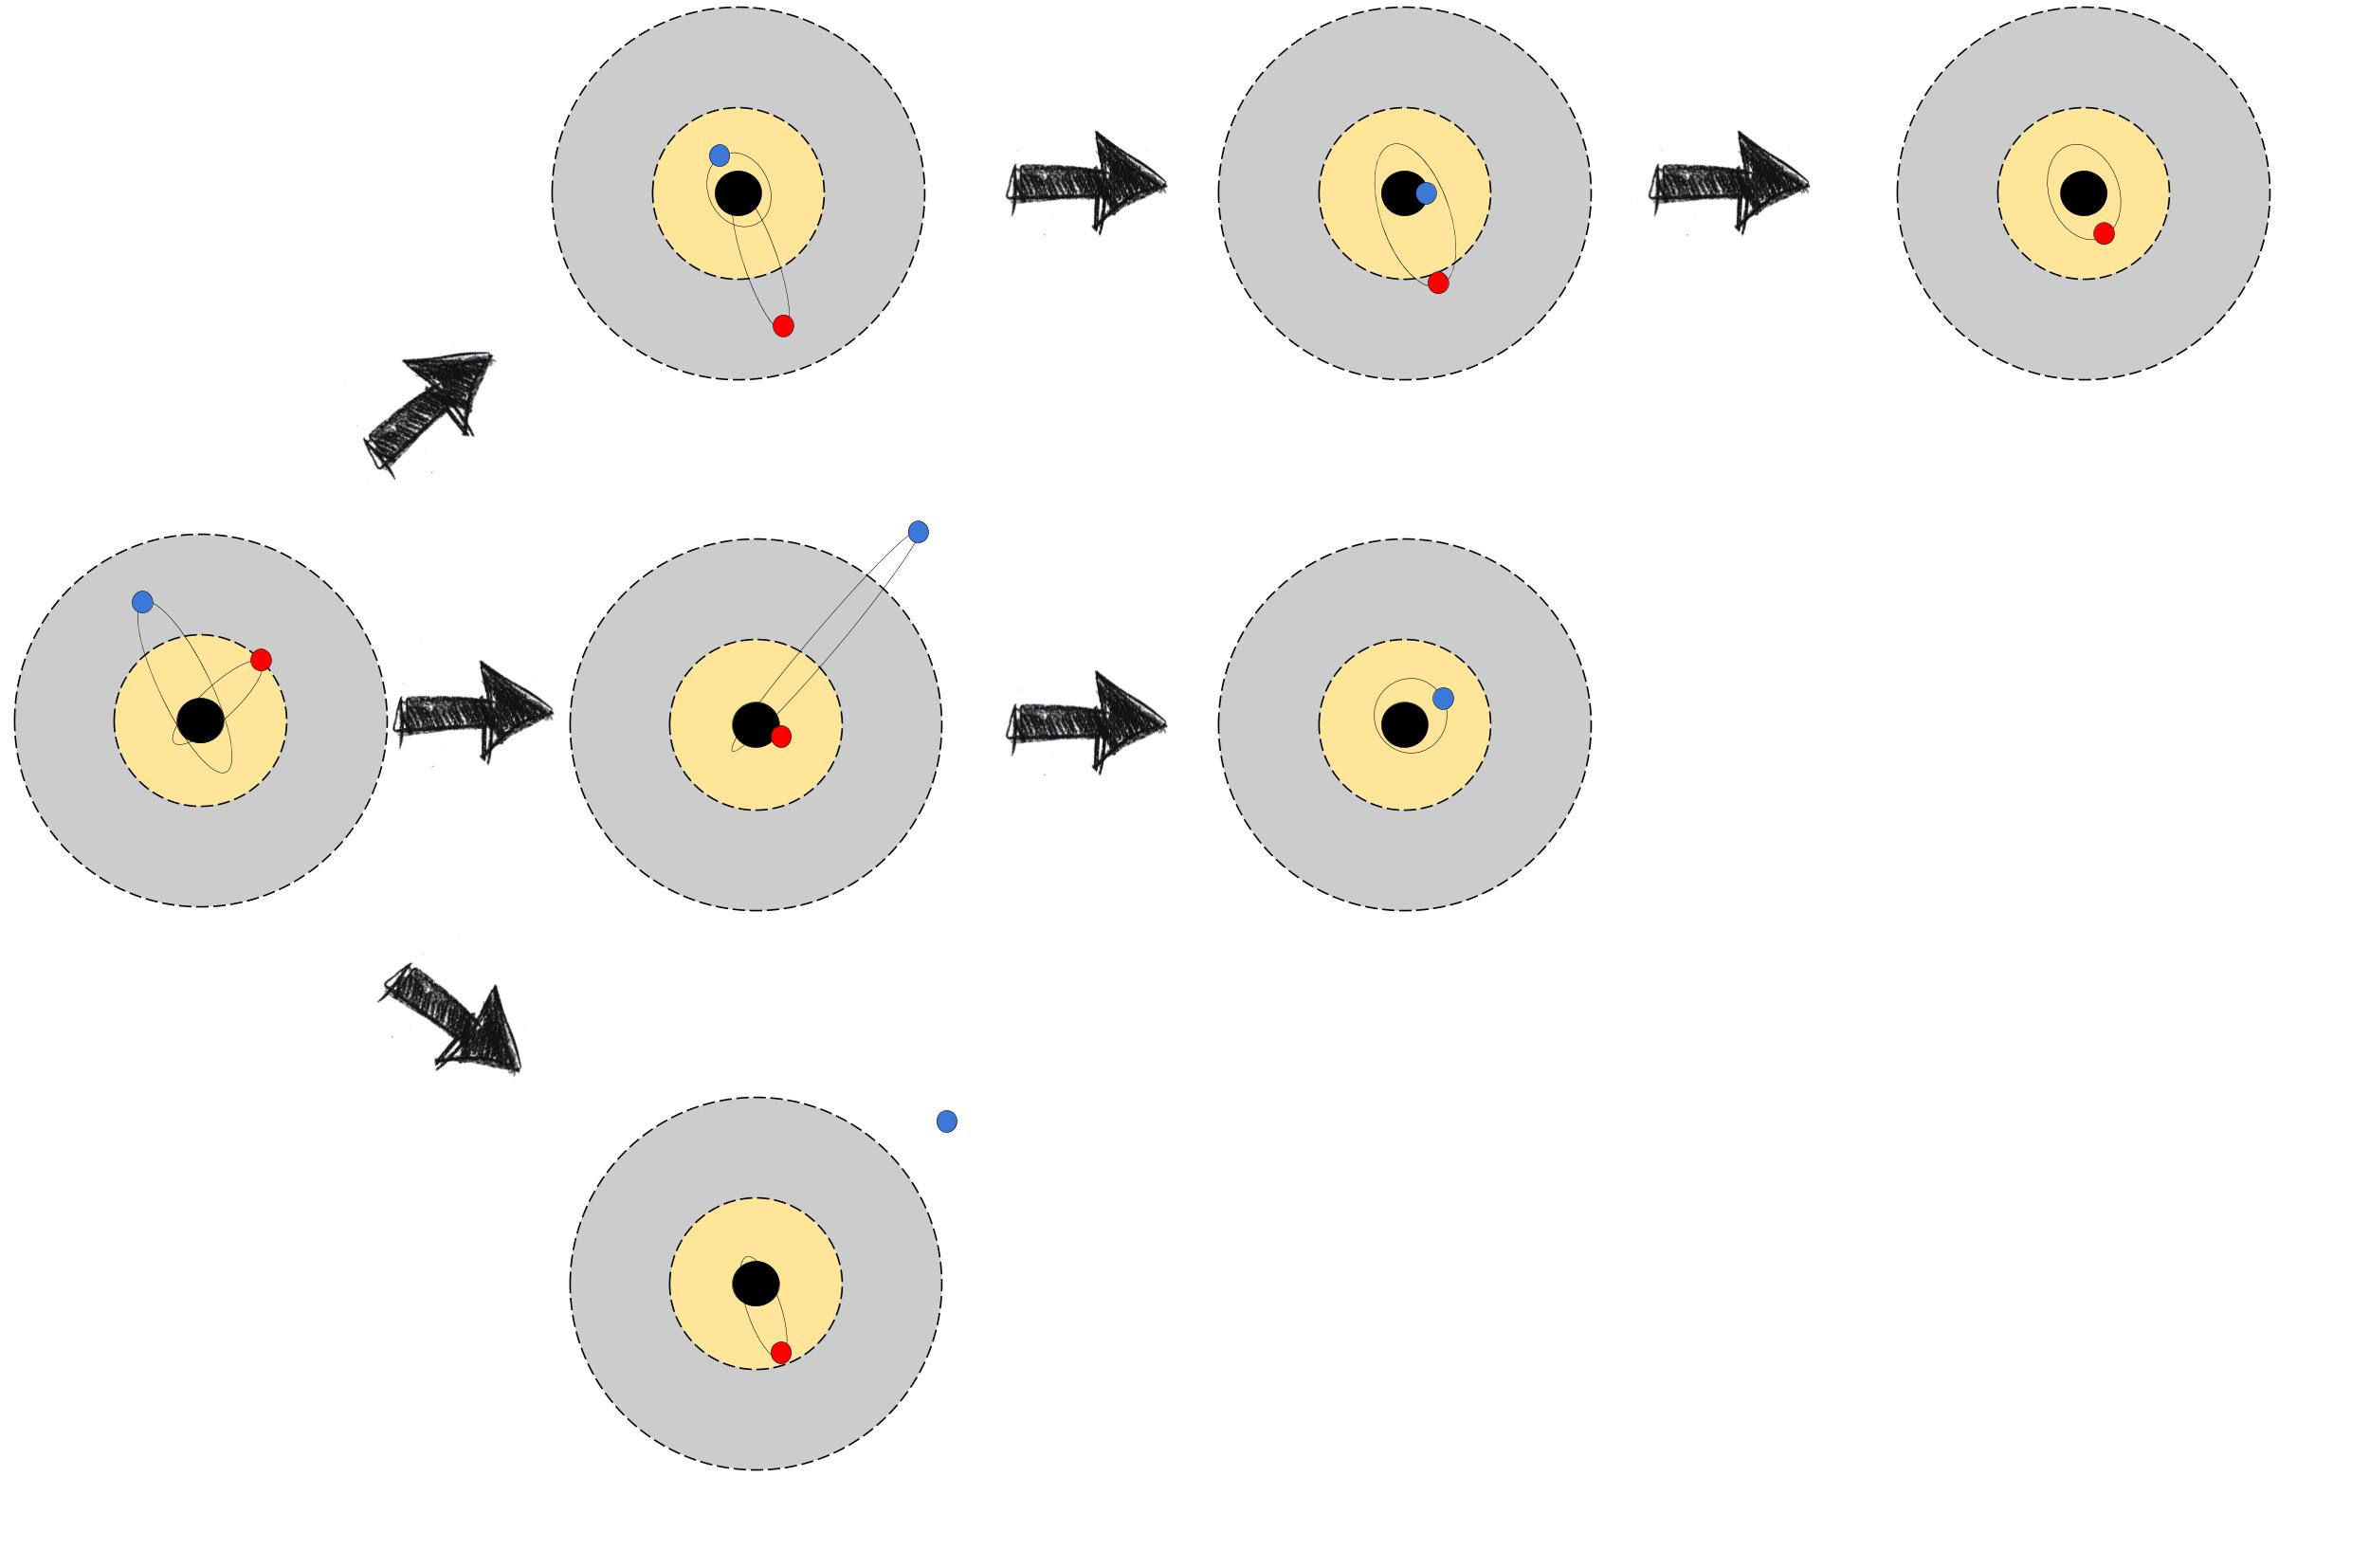
\includegraphics[width=12cm]{cases}
%\caption{Schematic view of the system.}
%\label{sketch}
%\end{figure*}


\section{Results}

In the simplest case in which a BH forms a bound binary with the IMBH and the interactions with passing-by stars is ineffective, the BH-IMBH will inspiral until coalescence over a time-scale \citep{peters64}
\begin{align}
t_\gw =&  \displaystyle \frac{5}{256}\frac{c^5 a_\inn^4 (1-e_\inn^2)^{7/2}}{G^3M_\ibh M_\bh(M_\ibh+M_\bh)} = \nonumber \\
       & 10^6{\rm ~yr}\left(\frac{a_\inn}{0.1\au}\right)^4\left(1-e_\inn^2\right)^{7/2}\times \nonumber \\ 
       & \times \left(\frac{10^3\Ms}{M_\ibh}\right) \left(\frac{30\Ms}{M_\bh}\right)\left(\frac{1030\Ms}{M_\ibh+M_\bh}\right).
\label{peters}
\end{align}
Note that in in our models, the most bound circular IMBH-BH pair ($a_\inn=10\au$) has a corresponding merger timescale of $\sim 10^{14}$ yr, due to the $\propto a_\inn^4$ dependence. Therefore, in order for an IMRI to develop, some external process is needed to shrink the binary sufficiently to enter in the GW-dominated regime. 

A third perturber can significantly affect the orbital evolution of the IMBH-BH binary. For instance, the three-body system can adjust itself in a hierarchical configuration, namely the outer BHs is sufficiently far to induce a secular perturbation on the inner binary, which might undergo a periodic oscillation of the eccentricity \citep[Kozai-Lidov oscillations]{lidov62,kozai62}, and eventually merge. As opposite to this, the inner and outer binaries have similar semi-major axis or periastron distances, and the evolution of the system is dominated by the chaotic nature of the BH-BH-IMBH interactions. Note that this process acts similarly to the so-called resonant scatterings that involve BHs or stars in dense clusters \citep{goodman93}.

A parameter that can be used to discern hierarchical systems is defined as \citep{Lithwick11,naoz11}
\begin{equation}
\epsilon = \frac{a_{\inn}}{a_{\out}}\frac{e_{\out}}{1-e_{\out}^2},
\end{equation}
being hierarchical those systems having $\epsilon<0.01$. In Figure \ref{F2}, we show the final merger time-scale as calculated through the \cite{peters64} formula as a function of the initial $\epsilon$ value for our models. We also highlight through colors the ratio between the final and initial merger time-scale for the inner binary. It turns out that the minimization of the merger time is achieved when $\epsilon \simeq 0.02-20$. Above this range the effect of the third object is less effective on the IMBH-BH evolution, whereas below this threshold the outer object is closer to the IMBH than the secondary BH, making difficult to define an inner and outer binary at all. We note that models with $\epsilon$ within the limits are not hierarchical, and their evolution is mostly determined by chaos. In a few cases, we find that the merger time decreases by up to 10 order of magnitude, leading the IMBH-BH to merge within $1 - 10^5$ yr.  

\begin{figure}
\centering
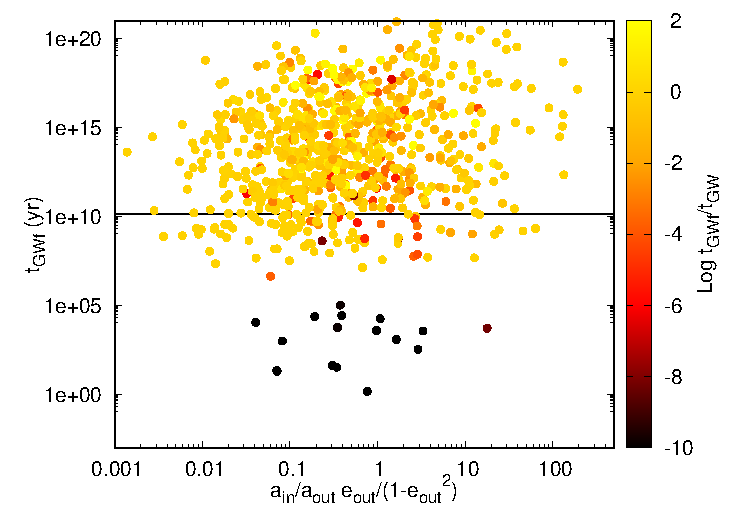
\includegraphics[width=8cm]{merger_hierarchy}
\caption{Final value of the inner binary merger time as a function of the hierarchy factor. Color coding identifies the ratio between the inner binary final and initial merger timescales. The horizontal line marks a merger time of $14$ Gyr.}
\label{F2}
\end{figure}

\begin{figure}
\centering 
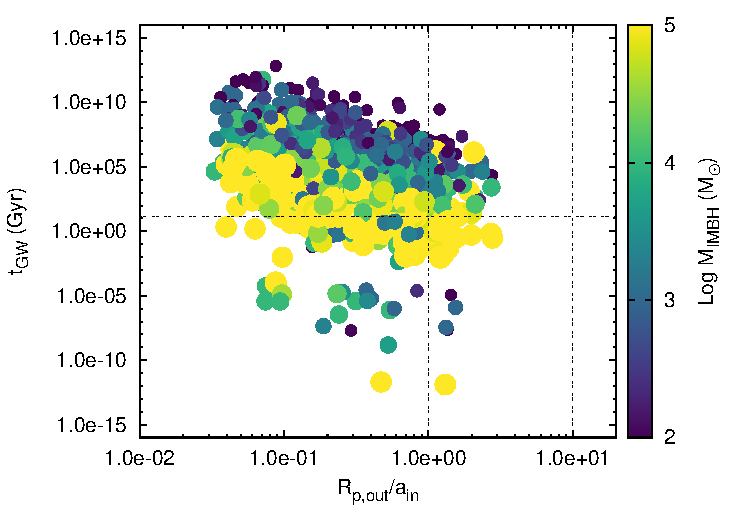
\includegraphics[width=8cm]{set15_res}
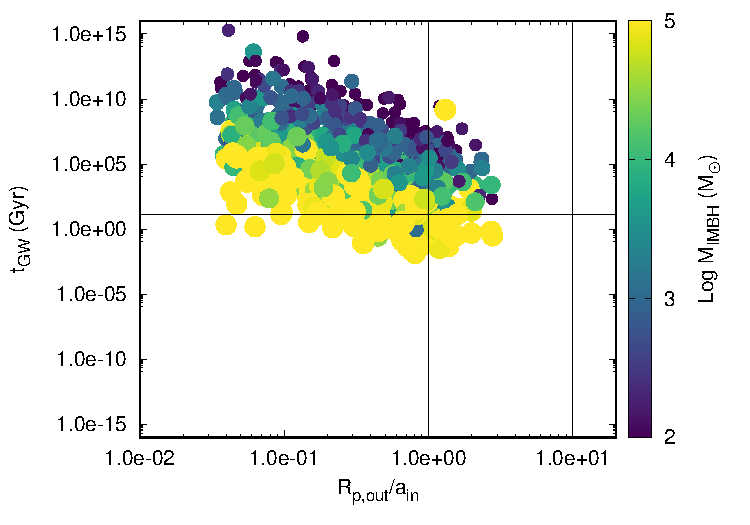
\includegraphics[width=8cm]{set15_res_init}
\caption{Final (top panel) and initial (bottom panel) value of the inner binary GW time-scale as a function of the ratio between the initial values of the outer pericentre and inner semi-major axis. The color-coding marks the IMBH mass.}
\label{res1}
\end{figure}

In order to estimate the number of mergers, we use Eq. \ref{peters} to calculate the merger timescale for the inner binary by the end of the simulation. Following this prescription, in model 1 the IMRI formation probability is $11.6\%$, while in model 2, where we assume a smaller range for the outer binary semi-major axis, the percentage rises up to $16.6\%$. Combining all the models together leads to an overall IMRIs probability of $14.2\%$.

The time distribution of the inner binary allows us to have a clean view on the effect that the outer object impinges on the inner binary evolution. Indeed, it is evident the formation of a small sample of systems with merger times below $10^5$ yr. These short-lived systems constitute the $2.8\%$ of the whole simulations, and are almost equally distributed between model 1 and model 2. Moreover, they seem not to depend on the IMBH mass. As shown above, the most effective parameters in determining such small merger times are the orbital properties of the inner and outer binaries.

\begin{figure}
\centering
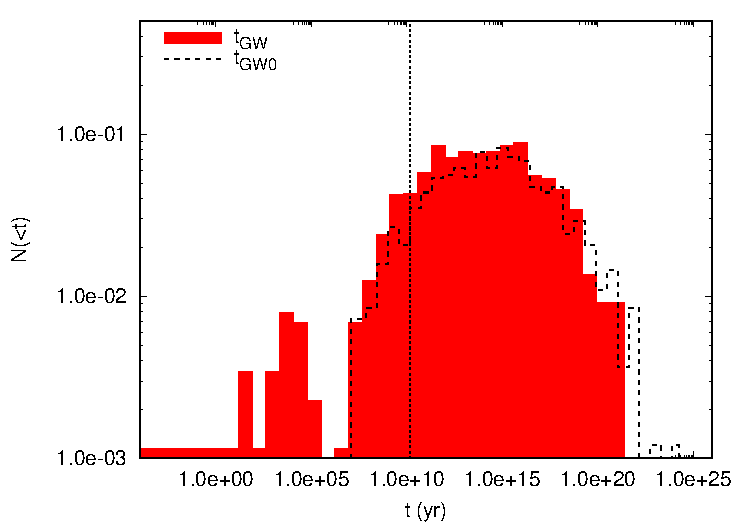
\includegraphics[width=8cm]{merger_time_histo}\\
\caption{Merger time distribution for the final (red filled boxes) and initial (black dotted steps) inner IMBH-BH binary. The vertical dotted line marks 14 Gyr.}
\label{F6}
\end{figure}

In order to understand whether the mergers population is characterized by peculiar orbital properties, we compare the final distribution of their semi-major axis and eccentricity with the corresponding initial values for the whole population, as shown in Figure \ref{F6}. 
We stress that both $a_{\rm mer}$ and $e_{\rm mer}$ are calculated from the last snapshot, thus they do not necessarily represent the binary orbital parameters promptly before the mergers. We postpone the discussion on the last stages of the IMRIs evolution to the next section.

The top panel shows clearly that the semi-major axis distribution of merging binaries differs significantly from the initial values, which is nearly uniform in the logarithms by assumption. The final distribution shows a peak at $\sim 10\au$, with a low-end extending down to $\lesssim 0.1 \au$. The eccentricity distribution, which is shown in the bottom panel, highlights that merging binaries tend to have a distribution steeper than the initial, thus implying that merger candidates are characterised by high eccentricities. Note that these distribution does not differentiate models with a different IMBH mass. In order to better understand the role played by the IMBH in determining the IMRI formation, we show in top panel of Figure \ref{F7} semi-major axis and eccentricity for merging systems in models 1 and 2 at varying the IMBH mass. Interestingly, all the mergers with $M_{\ibh} < 10^4\Ms$ have eccentricity above $0.9$. At larger IMBH mass values, instead, more than half of the models have smaller eccentricitities. 


\begin{figure}
\centering
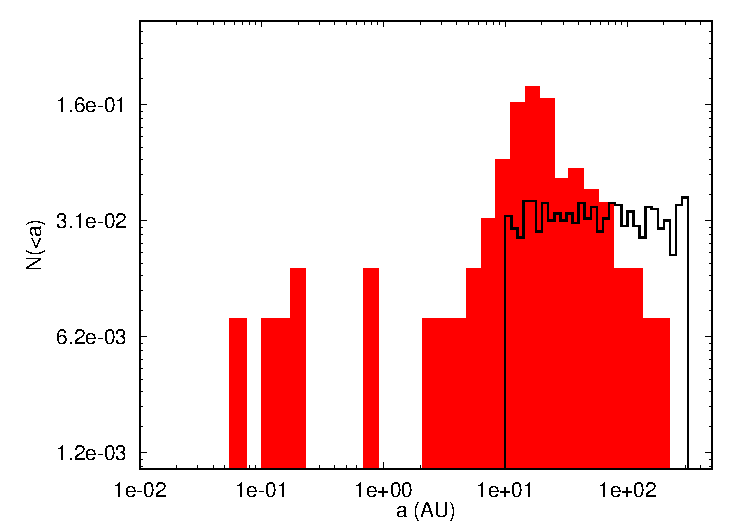
\includegraphics[width=8cm]{merger_semi_histo}\\
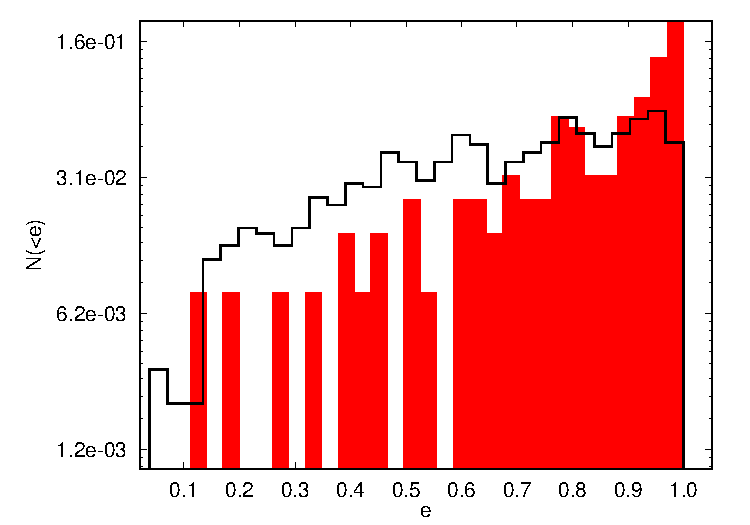
\includegraphics[width=8cm]{merger_ecce_histo}
\caption{Top panel: semi-major axis distribution for the inner binary. The black steps refer to initial values for all the simulations performed, while the red filled steps refer only to merger binaries and final values. Bottom panel: the same as in top panel, but for the inner binary eccentricity.}
\label{F6}
\end{figure}


This might have an interesting implication on the general properties of IMRIs developing in dense clusters. Indeed, since lighter clusters host, in general, lighter IMBHs, and since lighter IMBHs seem to be characterized by larger eccentricities, we would expect that the smaller the host cluster the larger the probability for an eccentric IMRIs to develop. Indeed, as shown in bottom panel of Figure \ref{F7}, the mean eccentricity for merging binaries as a function of the IMBH mass shows a decreasing trend, being $\langle e\rangle\sim 0.95$ at $M_{\ibh}\leq 10^3\Ms$ and steeply decreasing to $\langle e\rangle < 0.7$ at $M_{\ibh}\geq 8\times 10^4\Ms$.
\begin{figure}
\centering
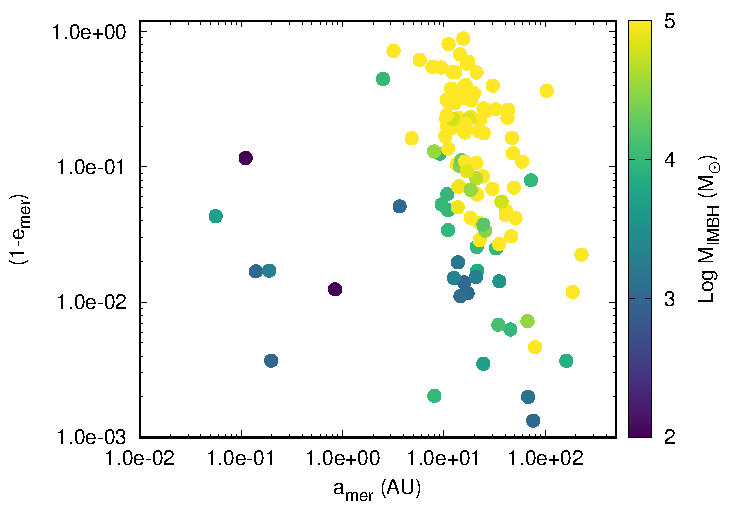
\includegraphics[width=\columnwidth]{mergers_distr}\\
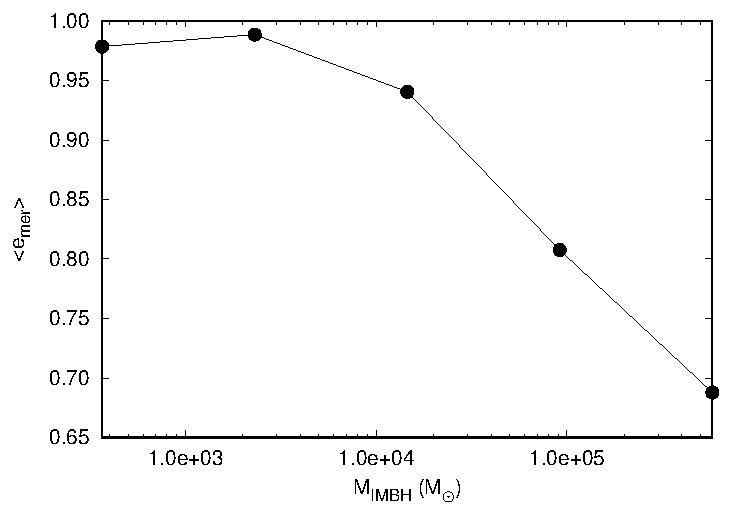
\includegraphics[width=8cm]{mean_ecce}\\
\caption{Top panel: The value complementary to the eccentricity ($1-e_{\rm mer}$) as a function of the semi-major axis ($a_{\rm mer}$) calculated at the last snapshot for all the merging binaries in all models. The coloured map identifies the IMBH mass. Bottom panel: mean eccentricity calculated in different IMBH mass bins, as a function of the IMBH mass for all mergers in both model 1 and 2.}
\label{F7}
\end{figure}

Figure \ref{res1} shows the inner binary merging time-scale as a function of the ratio between the outer pericentre and the inner semi-major axis, $R_{\rm p,\out} / a_\inn$, for all the simulations ran. Note that the merger time decreases at increasing this quantity, and that the minimum merger time is achieved when $R_{\rm p, \out} \simeq a_\inn$. It is trivial to note that at fixed $R_{\rm p,\out} / a_\inn$, the merger time decreases at increasing the IMBH mass due to the $t_\gw-M_\ibh$ dependence. This inevitably translates into a relatively strong dependence between the IMRIs formation probability $f_{\rm mer}$ and the IMBH mass. Indeed, our simulations show that the lower the IMBH mass the lower the probability for IMRIs to form. Figure \ref{F5} shows how $f_{\rm mer}$ varies with $M_{\ibh}$ for model 1 and 2 and for the total sample. 
The difference between the two models increase abruptly at IMBH masses above $10^5\Ms$, where the effect of an initially tighter outer BH leads the IMRIs number to increases sizably. The merger probability can be represented with a power-law of the form
\begin{equation}
f_{\rm mer} = \alpha \left(\frac{M_\ibh}{10^2\Ms}\right)^\beta,
\end{equation}  
with the fitting values summarized in Table \ref{t2}. 
Our simulations suggest that whenever a three-body encounter occurs in a GC containing a $10^4\Ms$ IMBH, there is a $\sim 10\%$ of the probability for IMRIs formation and the eccentricity at formation is of the order of 0.95. 

In the next section we discuss the last phase of evolution for merging pairs in our simulations.

\begin{figure}
\centering 
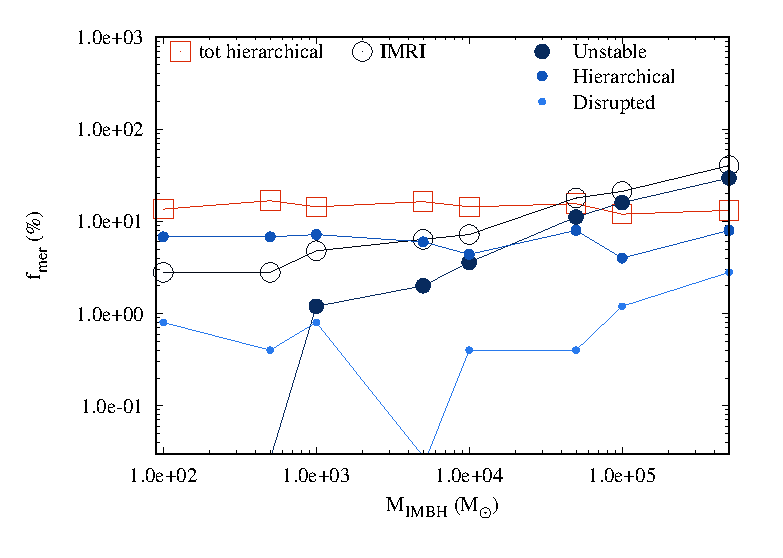
\includegraphics[width=8cm]{mergers}
\caption{Percentage of mergers as a function of the IMBH mass for all the models (black dots), model 1 (blue squares) or model 2 (red triangles).}
\label{F5}
\end{figure}

\begin{table*}
\caption{Fitting parameters for merger probability}
\begin{center}
\begin{tabular}{ccccc}
\hline
\hline
model & $\alpha$ & $\beta$ & $f_{\rm mer}(10^2\Ms)$ & $f_{\rm mer}(10^4\Ms)$  \\
      & & & $(\%)$ & $(\%)$ \\
\hline
1   & $1.73\pm 0.45$& $0.22\pm 0.02$& $4.7$& $12.6$\\
2   & $0.81\pm 0.68$& $0.28\pm 0.07$& $3.0$& $11.1$\\
all & $0.69\pm 0.32$& $0.29\pm 0.04$& $2.7$& $10.5$\\
\hline
\end{tabular}
\end{center}
\label{t2}
\end{table*}





\section{Gravitational waves}

As stated in the previous sections, we find a total number of 130 mergers out of the 928 simulations performed, irrespectively of the assumed initial conditions. 


Among all the runs performed, we find two interesting cases, namely s151 and s400, in which the stellar mass BHs are initially sufficiently close to form a tight binary. In both cases, the IMBH mass is relatively small $M_{\ibh} = 100\Ms$, and the inner binary is comprised of the other two, stellar-mass, BHs. It is not surprising that a BH-BH pair forms in a model with low-mass IMBH, due to the lower velocity dispersion and the larger tidal radius needed for the binary to form without being ripped apart from the IMBH. In both cases, the BH-BH binary undergoes Kozai-Lidov oscillations, which periodically induce an increase in the binary eccentricity and the mutual inclination.

In model s400, the amplitude of the oscillation is minimal, the mutual inclination ranges between $i = 126-130^\circ$, while the eccentricity varies in the range $e = 0.882-0.904$. Although the KL effect is not very efficient in affecting the BH-BH evolution, the binary is sufficiently tight to have a short merger timescale, being $t_{\rm gw} \simeq 3\times 10^7$ yr.

In model s151, instead, the Kozai-Lidov effect is more effective, leading the inclination to vary strongly in the range $\sim 40-90^\circ$ and the eccentricity to rise up to $e = 0.99$. The time evolution of both $e$ and $i$ is shown in Figure \ref{F9}, together with the associated merger time-scale. 
Due to the cyclic increase in $e$, which leads to episodic GW bursts, the merger time will be reduced by a factor proportional to the maximum eccentricity, more precisely \citep{antonini12}
\begin{equation}
t_{\gw, \rm eff} = t_{\gw}(a_0,e_0) \frac{\left(1-e_{\rm max}^2\right)^{7/2}}{\left(1-e^2\right)^{7/2}},
\end{equation}
being $t_{\gw}(a_0,e_0)$ the merger time calculated at time zero. In this particular simulation, the inner binary achieves a maximum eccentricity value of $e_{\rm max} = 0.99$, thus implying a merger time $\sim 2.4\times 10^7$ yr, i. e. $5600$ times smaller than the time needed for the same binary to merge in isolation.

We find these BH-BH binaries only in the subset of simulations in model 1 where we set $M_\ibh = 100\Ms$. Assuming that BH-BH binary formation is favoured only in the case of IMBH with ``low'' masses, we can infer a formation probability for stellar-mass binaries to be $\sim 2\%$. 


\begin{figure}
\centering 
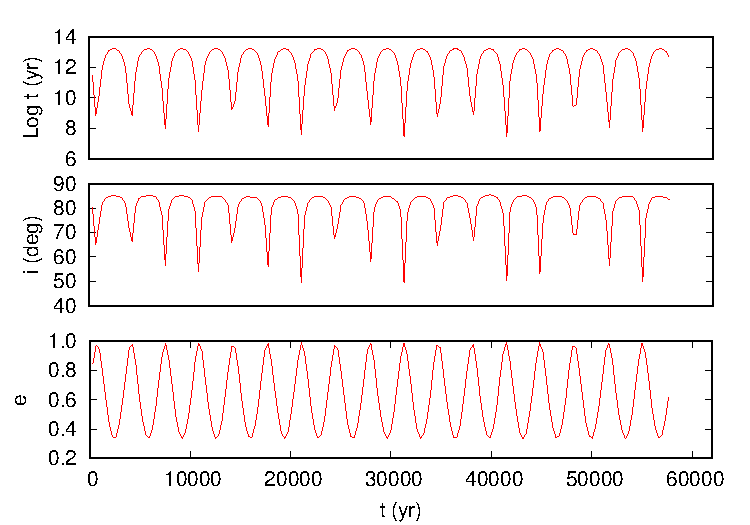
\includegraphics[width=8cm]{kozai_151}
\caption{Top panel: time evolution of the merger timescale for model number 151, in which two BHs pair together while the IMBH acts as a perturber. Central panel: mutual inclination as a function of time for the BH-BH pair in simulation number 151. Bottom panel: ecentricity as a function of time for the BH-BH pair in simulation number 151.}
\label{F9}
\end{figure}

In all the other cases, the merging binary is comprised of the IMBH and one of the two BHs. After the IMBH-BH enters the GW-dominated regime, its subsequent evolution is not subjected to external perturbers anymore \citep{seoane18}. In order to obtain information about the GW properties of these mergers, we took the IMBH-BH binaries orbital parameters from the last output in simulations and calculated the following evolution of semi-major axis and eccentricity following \cite{peters64}. As long as the binary preserve a residual eccentricity, the GW signal is audible in a range of frequency, rather than being a monochromatic emission. The peak frequency can be approximated as \citep{wen03, antonini12}
\begin{equation}
f_\gw = \frac{1}{\pi}\sqrt{\frac{GM_{\rm bin}}{a^3}}\frac{\left(1+e\right)^{1.1954}}{\left(1-e^2\right)^{3/2}},
\end{equation}  
being $M_{\rm bin}$ the merging binary total mass. Using this definition, we show in Figure \ref{F10} how the peak frequency and eccentricity vary for mergers in our models. In order to understand whether these sources can be audible to GW observatories, we superpose our calculations to the observational windows of the Laser Interferometer Space Antenna \citep[LISA\footnote{\url{https://www.elisascience.org/}},][]{amaro12}, the Deciherz Gravitational-Wave Observatory \citep[DECIGO\footnote{\url{http://tamago.mtk.nao.ac.jp/spacetime/decigo_e.html}},][]{seto01}, and the Einstein Telescope \citep[ET\footnote{\url{http://www.et-gw.eu/}},][]{punturo10}. 

\begin{figure}
\centering
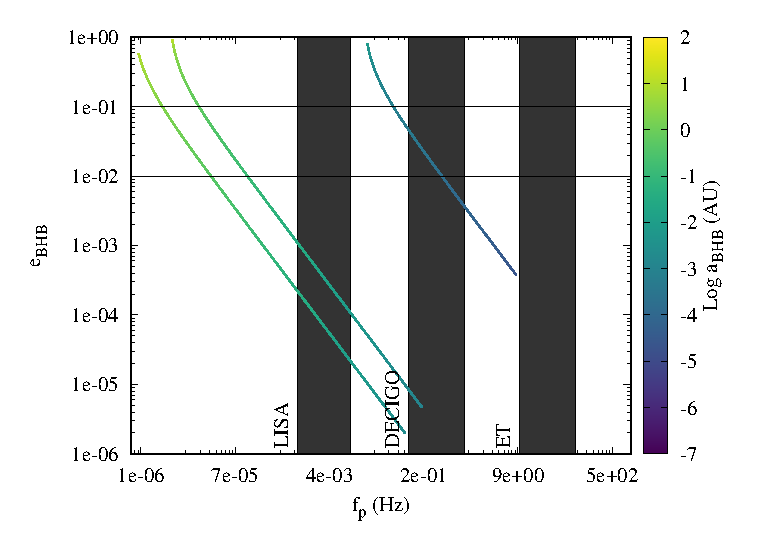
\includegraphics[width=8cm]{freq_evo}\\
\caption{Frequency (x-axis) and eccentricity (y-axis) evolution for merging binaries in our models. The color coding identifies the semi-major axis evolution. The black boxes identify the observational windows of LISA, DECIGO and the Einstein Telescope. The horizontal lines mark two values of the eccentricity, namely $e=0.01-0.1$.}
\label{F10}
\end{figure}

It is interesting to note that a handful of sources could have a non-negligible eccentricity both in the LISA and DECIGO observational band, while at larger frequencies the binaries are already completely circular. In order to better highlight the probability for low-frequency detectors to observe eccentric IMRIs, we show in Figure \ref{F11} the eccentricity distribution of sources entering the mHz and Hz frequency bands. We find that only $2\%$ of sources have high eccentricity in the LISA band, while for DECIGO this quantity is slightly larger ($\sim 7\%$) and the majority of mergers, $\sim 20\%$ have $e\sim 0.02$.

\begin{figure}
\centering
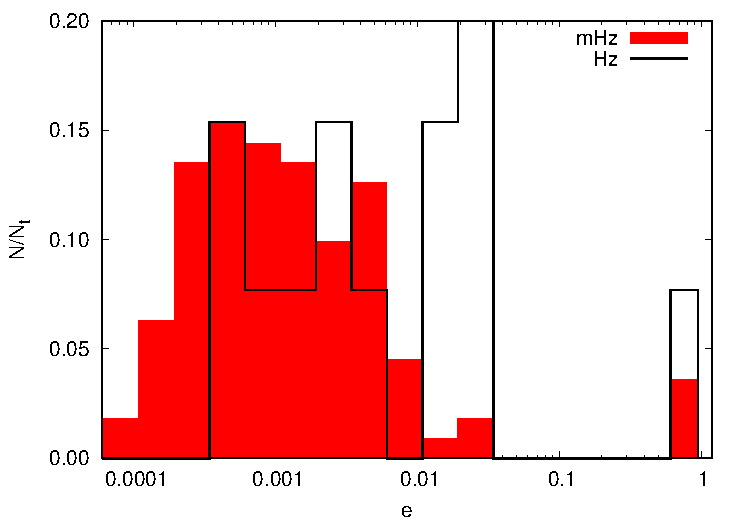
\includegraphics[width=8cm]{ecc_distri_merge}\\
\caption{Eccentricity distribution for IMRIs in our models. The eccentricity is calculated at the moment in which a source cross the mHz (red filled steps) or Hz frequency band (black steps).}
\label{F11}
\end{figure}



{\bf PERHAPS PAU CAN CALCULATE THE STRAIN OF THE DOMINANT FREQUENCY JUST TO COMPARE TO NEXT FIGURE...}

In order to calculate understand whether these sources might be audible to GW observatories, we calculated the strain following \cite{kocsis12} for all the frequencies containing the $95\%$ of the emitted power. We assume a luminosity distance $D_L = 100$ Mpc and redshift $z=0.11$, and a 5 yr observation time. Figure \ref{F12} shows the evolution of the strain-frequency evolution for two different mergers, altogether with the eccentricity decrease due to GW circularization. For the sake of visibility, we only show the strain associated to the dominant frequency. In the two models shown in the plot, the mergers outshine in the LISA band, where they spend most of their life, and slowly shift toward higher frequency, merging inside the LIGO observational band. These sources are of extreme interest since they can be used to further constrain and test the General Relativity theory, as their evolution can be monitored in both the low- and high-frequency regime. {\bf ADD SOME TEXT?}


\begin{figure}
\centering
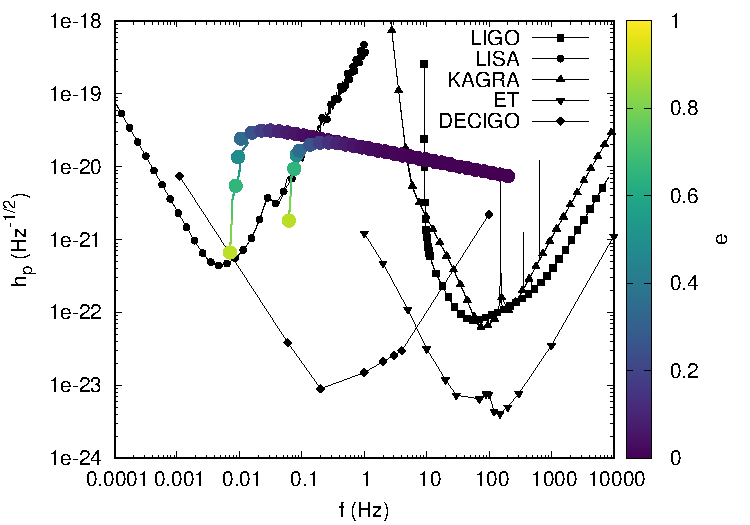
\includegraphics[width=8cm]{strain_n21}\\
\caption{Strain calculated for the dominant frequency for two different models, assuming an infinite observational time. We overlap the simulated data with sensitivity curves from several GW observatories.}
\label{F12}
\end{figure}

\section{Conclusions}
\begin{itemize}

\item we study the formation and evolution of IMRIs in globular clusters using three-body experiments;
\item we show that the presence of a perturber can greatly increase IMRIs formation probability, reducing significantly the IMRIs semi-major axis and increasing its eccentricity;
\item we find that the IMRIs formation probability increases at increasing the IMBH mass, being $\sim 10-15\%$ for typical IMBH ($M_\ibh = 10^4\Ms$);
\item the population of IMRIs that form in our models are characterised by a well defined semi-major axis distribution that peaks at $10\au$ and deviates significantly from the assumed initial configuration. The eccentricity distribution is steeper than the standard thermal distribution, thus implying that IMRIs preferentially form in nearly radial configurations;
\item the average eccentricity calculated during the IMRIs formation seems to depend on the IMBH mass, being larger for lighter IMBHs. Our models suggest that IMRIs with IMBHs in the low-end of the mass distribution, $M_\ibh \simeq 10^2-10^3\Ms$, are most likely characterized by eccentricities above 0.95, whereas heavier IMBHs lead to the formation of IMRIs having more moderate eccentricity values, $\langle e\rangle \lesssim 0.8$.
\item we find that in the case of low-mass IMBHs ($M_\ibh \sim 100\Ms$) stellar mass BHs can pair, although this formation channel is disfavoured, being the occurrence only of $2\%$. In one of the cases examined, the BH-BH binary and the IMBH arrange themselves in a triple configuration. The BH-BH evolution is mostly determined by Kozai-Lidov oscillations induced by the IMBH, which leads the BH-BH to merge over a relatively short timescale ($2.4\times 10^7$ yr).
\item we calculated the semi-major axis, eccentricity and GW frequency evolution for all the IMRIs in our models, showing that they might be audible to both low- and high-frequency detectors. A handful of them could show up in the LISA and DECIGO bands as eccentric sources, while the vast majority of mergers in our models are already circular when crossing the mHz frequency window. In a few cases, we find that an IMRIs appears in the LISA band first and due to the inspiral crosses all the detectors observational windows until they merge in the LIGO band.  

\end{itemize}

\section*{Acknowledgements}

Sonderforschungsbereich SFB 881 "The Milky Way System" (subproject Z2) of the German Research Foundation (DFG) for the financial support provided. This work benefited of financial support from the Alexander von Humboldt Foundation, which granted MAS research program ``The evolution of black holes from stellar to galactic scales''. 
This work benefited from support by the ISSI (Bern), through its Intern. Team prog. ref. no. 393 {\it The Evolution of Rich Stellar Populations \& BH Binaries} (2017-18).


\footnotesize{
\bibliographystyle{mn2e}
\bibliography{ASetal2015}
}



\end{document}